\documentclass[11pt,a4paper]{article}

% ---------- Packages ----------
\usepackage[utf8]{inputenc}
\usepackage[T1]{fontenc}
\usepackage[margin=1in]{geometry}
\usepackage{xcolor}
\usepackage{titlesec}
\usepackage{enumitem}
\usepackage{setspace}
\usepackage{hyperref}
\usepackage{fancyhdr}
\usepackage{graphicx}

% ---------- Math ----------
\usepackage{amsmath}
\usepackage{amssymb}
\usepackage{amsfonts}

% ---------- Colors ----------
\definecolor{headingblue}{RGB}{31,56,100}
\definecolor{subheadingblue}{RGB}{46,83,149}
\definecolor{graytext}{RGB}{85,85,85}

% ---------- Section styling ----------
\titleformat{\section}
{\normalfont\Large\bfseries\color{headingblue}}{\thesection}{1em}{}
\titleformat{\subsection}
{\normalfont\large\bfseries\color{subheadingblue}}{\thesubsection}{1em}{}

% ---------- Header/footer ----------
\pagestyle{fancy}
\fancyhf{}
\fancyfoot[C]{\thepage}
\renewcommand{\headrulewidth}{0pt}

% ---------- Hyperref setup ----------
\hypersetup{
	colorlinks=true,
	linkcolor=headingblue,
	citecolor=headingblue,
	urlcolor=headingblue,
	pdftitle={mRNA Secondary Structure Prediction via Quantum Optimization},
	pdfauthor={Pushkar Kumar and Harold Ohandja}
}

\setstretch{1.15}

\begin{document}
	
	% =========================================================
	% COVER PAGE
	% =========================================================
	\begin{titlepage}
		\centering
		\vspace*{2.5cm}
		
		{\bfseries\color{graytext} WISER GLOBAL QUANTUM+AI PROGRAM 2026}\\[0.2cm]
		{\bfseries\color{graytext} WISER $\times$ Moderna Challenge}
		
		\vspace{0.4cm}
		\noindent\rule{\textwidth}{0.4pt}
		\vspace{2cm}
		
		{\Huge\bfseries mRNA Secondary Structure Prediction via Quantum Optimization\par}
		
		\vspace{0.8cm}
		{\Large\itshape\color{graytext} A QUBO Formulation Solved with CVaR-VQE, Benchmarked Against the ViennaRNA MFE\par}
		
		\vspace{2.5cm}
		
		{\large\bfseries Team}\\[0.3cm]
		{\large Pushkar Kumar --- Lead: Quantum/ML Formulation \& Implementation}\\[0.15cm]
		{\large Harold Ohandja --- Classical Solvers, Benchmark Automation \& Resource Analysis}
		
		\vspace{2.5cm}
		
		{\large Submitted August 7, 2026}\\[0.15cm]
		{\color{graytext} WISER Quantum 2026 --- The Washington Institute for STEM, Entrepreneurship and Research}
		
		\vfill
		
		{\color{graytext}\small Live interactive demo: \url{https://harold-ohandja.github.io/Moderna-Quantum-RNA-/}}
	\end{titlepage}
	
	% =========================================================
	% ABSTRACT
	% =========================================================
	\section*{Abstract}
	\addcontentsline{toc}{section}{Abstract}
	
	The secondary structure of messenger RNA (mRNA) directly influences its stability, translation efficiency, and manufacturability, making it a critical parameter in the design of mRNA-based therapeutics. Predicting this structure amounts to solving a combinatorial optimization problem whose search space grows exponentially with sequence length; the general problem, when pseudoknots are included, is NP-hard. Classical tools such as ViennaRNA rely on dynamic programming to approximate the lowest free-energy structure (Minimum Free Energy, MFE), but remain limited when it comes to exploring the broader energy landscape or incorporating richer structural constraints.
	
	This project, carried out as part of the WISER $\times$ Moderna challenge (WISER Global Quantum+AI Program 2026), formulates mRNA secondary-structure prediction as a Quadratic Unconstrained Binary Optimization (QUBO) problem and solves it using a hybrid quantum-classical variational algorithm, CVaR-VQE (Conditional Value at Risk -- Variational Quantum Eigensolver), following the approach proposed by Alevras et al. (IBM Quantum \& Moderna, 2024). The binary variables of the QUBO represent candidate base-pairings; the objective function approximates the folding free energy, and penalty terms enforce non-crossing and compatibility constraints between selected pairs. The structures produced by this approach are compared against the reference MFE structure obtained via ViennaRNA, both in terms of energy gap and structural similarity.
	
	The work covers: (i) a literature review of existing QUBO formulations for RNA folding; (ii) the construction of a classical benchmarking harness based on ViennaRNA, together with two independent classical baselines (exact brute-force and a greedy heuristic); (iii) the implementation of CVaR-VQE with a hardware-efficient \texttt{n\_local} ansatz and the COBYLA classical optimizer on short sequences (8--10 nucleotides); (iv) an analysis of how quantum resource requirements (qubit count, circuit depth, runtime) scale with sequence length, reported both as a theoretical upper bound and as empirical measurements; and (v), as bonus tasks, an explicit justification for excluding pseudoknots, a comparison against a QAOA approach on the same problem instance, and a noise-robustness study under simulated shot and depolarizing noise. The goal is not to outperform classical methods, but to reproduce known reference structures for small sequences and characterize how quantum resource requirements scale with problem size. A central, honestly reported finding is that on some sequences every method---including exhaustive brute force---fails to match the reference, isolating a limitation of the simplified QUBO energy model rather than of the quantum optimizer.
	
	\vspace{0.3cm}

	
	\clearpage
	
	% =========================================================
	% SECTION 1 -- INTRODUCTION
	% =========================================================
	\section{Introduction}
	
	\subsection{Biological and Industrial Context}
	
	Messenger RNA (mRNA) occupies a central place in the central dogma of molecular biology: it carries genetic information from DNA to the translation machinery, where it is converted into protein. Beyond its primary sequence (the string of nucleotides A, U, C, G), RNA folds onto itself through base pairing to form a secondary structure---helices, hairpin loops, bulges, internal loops, multi-branched junctions, and, in some cases, pseudoknots. This structure governs essential properties of the mRNA: its thermodynamic stability, its translation efficiency, its resistance to degradation, and, ultimately, its manufacturability at industrial scale.
	
	Moderna, whose therapeutic platform is built entirely around mRNA, has a direct interest in better predicting and controlling these structures during the design of its drug candidates. It is in this context that Moderna and the Washington Institute for STEM, Entrepreneurship and Research (WISER) proposed, as part of the WISER Global Quantum+AI Program 2026, a challenge to investigate whether quantum or quantum-inspired optimization methods can contribute to mRNA secondary-structure prediction.
	
	\subsection{Computational Problem}
	
	From a computational standpoint, predicting the secondary structure of an RNA molecule amounts to searching, among all physically valid base-pairings, for the configuration that minimizes the molecule's free energy---the so-called Minimum Free Energy (MFE) structure. The number of possible structures grows very rapidly with sequence length, and the problem becomes NP-hard once complex structures such as pseudoknots are allowed. Classical reference tools such as ViennaRNA circumvent this difficulty through dynamic-programming algorithms (in the tradition of Zuker and Nussinov) that efficiently find the MFE structure as long as pseudoknots are excluded from the model; exhaustively exploring the full energy landscape, however, remains beyond the reach of these approaches.
	
	This combination---a cost function that is quadratic in the pairing variables, together with the need to enforce compatibility constraints between pairs---makes the problem naturally amenable to a Quadratic Unconstrained Binary Optimization (QUBO) formulation. A QUBO, in turn, can be encoded as an Ising Hamiltonian and solved using quantum algorithms, whether on quantum annealers or on gate-based quantum computers. This bridge is what motivates the still-emerging interest in quantum computing for this problem.
	
	\subsection{Related Work and Positioning}
	
	Several QUBO formulations of the RNA folding problem have already been proposed in the literature, notably by Fox et al. (2022), who define variables at the level of stems or stacked quartets, and by Zaborniak et al. (2022), who refine these models using a variational hybrid quantum annealing approach trained on known structures. The work most directly relevant to this challenge, however, is that of Alevras, Metkar, Yamamoto, Kumar et al. (IBM Quantum \& Moderna, 2024), who formulate the problem as a QUBO at the level of stacked base-pair quartets and solve it with CVaR-VQE on IBM Eagle and Heron quantum processors, for sequences of up to 42 nucleotides (10 to 80 qubits). Their results reproduce MFE structures identical to those obtained with the classical solver CPLEX, even on noisy quantum hardware, which constitutes an important proof of feasibility.
	
	This project adopts this approach as its primary method: a QUBO formulation over candidate base pairs, solved with CVaR-VQE using a hardware-efficient \texttt{n\_local} ansatz and a gradient-free classical optimizer (COBYLA), validated on shorter sequences (on the order of 8--10 nucleotides) compatible with the local-simulation resources available for this challenge.
	
	\subsection{Project Objectives}
	
	In line with the challenge statement, this project pursues the following objectives:
	
	\begin{itemize}[leftmargin=1.2cm]
		\item Formulate mRNA secondary-structure prediction as a QUBO optimization problem, with binary variables representing candidate base-pairings and penalty terms enforcing non-crossing and pairwise compatibility.
		\item Generate reference MFE structures using ViennaRNA for short synthetic sequences, and evaluate the energy of any candidate structure relative to this reference.
		\item Implement a quantum solver (CVaR-VQE) and compare the resulting structures and energies to the classical reference, reporting accuracy, energy gap, runtime, and observed limitations.
		\item Analyze how qubit count, circuit depth, and runtime scale with sequence length, in order to identify the point at which local simulation becomes impractical.
		\item As bonus tasks: justify the exclusion of pseudoknots from the initial model, compare the CVaR-VQE formulation against a QAOA approach on the same problem instance, and evaluate robustness under simulated sampling and depolarizing noise.
	\end{itemize}
	
	\subsection{Report Structure}
	
	The remainder of this report is organized as follows. Section~\ref{sec:background} presents the theoretical background: dot-bracket notation, the free-energy model, and a comparative review of existing QUBO formulations for RNA folding. Section~\ref{sec:formulation} details the QUBO formulation adopted for this project. Section~\ref{sec:methodology} describes the methodology and implementation, including the ViennaRNA benchmarking harness and the CVaR-VQE pipeline. Section~\ref{sec:results} presents the results obtained on the tested sequences, compared against the MFE reference. Section~\ref{sec:scaling} analyzes the scaling of quantum resource requirements, contrasting a theoretical upper bound with empirical measurements. Section~\ref{sec:discussion} discusses the limitations of the approach and the bonus tasks explored (pseudoknot exclusion, comparison with QAOA, and noise robustness). Section~\ref{sec:conclusion} concludes and outlines directions for future work.
	
	\clearpage
	
	% =========================================================
	% SECTION 2 -- THEORETICAL BACKGROUND AND RELATED WORK
	% =========================================================
	\section{Theoretical Background and Related Work}
	\label{sec:background}
	
	\subsection{RNA Secondary Structure and Representation}
	
	An RNA sequence is a linear polymer composed of four types of ribonucleotides: Adenine (A), Uracil (U), Cytosine (C), and Guanine (G). In an aqueous cellular environment, intramolecular hydrogen bonds form between non-adjacent complementary bases, causing the single-stranded chain to fold into a spatial configuration. Secondary structure refers to the ensemble of base pairs formed within the molecule.
	
	Valid base pairs typically include the standard Watson-Crick pairs ($\text{A--U}$, $\text{C--G}$) and the weaker wobble pair ($\text{G--U}$). Thermodynamically, secondary structures are composed of distinct structural motifs, as illustrated in Figure~\ref{fig:rna_motifs}:
	\begin{itemize}[leftmargin=1.2cm]
		\item \textbf{Helices (Stems):} Consecutive, stacked base pairs that stabilize the molecule through base-stacking interaction energy.
		\item \textbf{Hairpin Loops:} Unpaired regions enclosed by a single base pair at the end of a stem.
		\item \textbf{Internal Loops and Bulges:} Unpaired nucleotides breaking the continuity of a double helix.
		\item \textbf{Multi-branched Junctions:} Regions where three or more double-stranded stems meet.
		\item \textbf{Pseudoknot Motifs:} Non-nested tertiary/secondary interactions involving crossing base pairs (excluded from our initial model; see Section~\ref{sec:formulation}).
	\end{itemize}
	
	\begin{figure}[htbp]
		\centering
		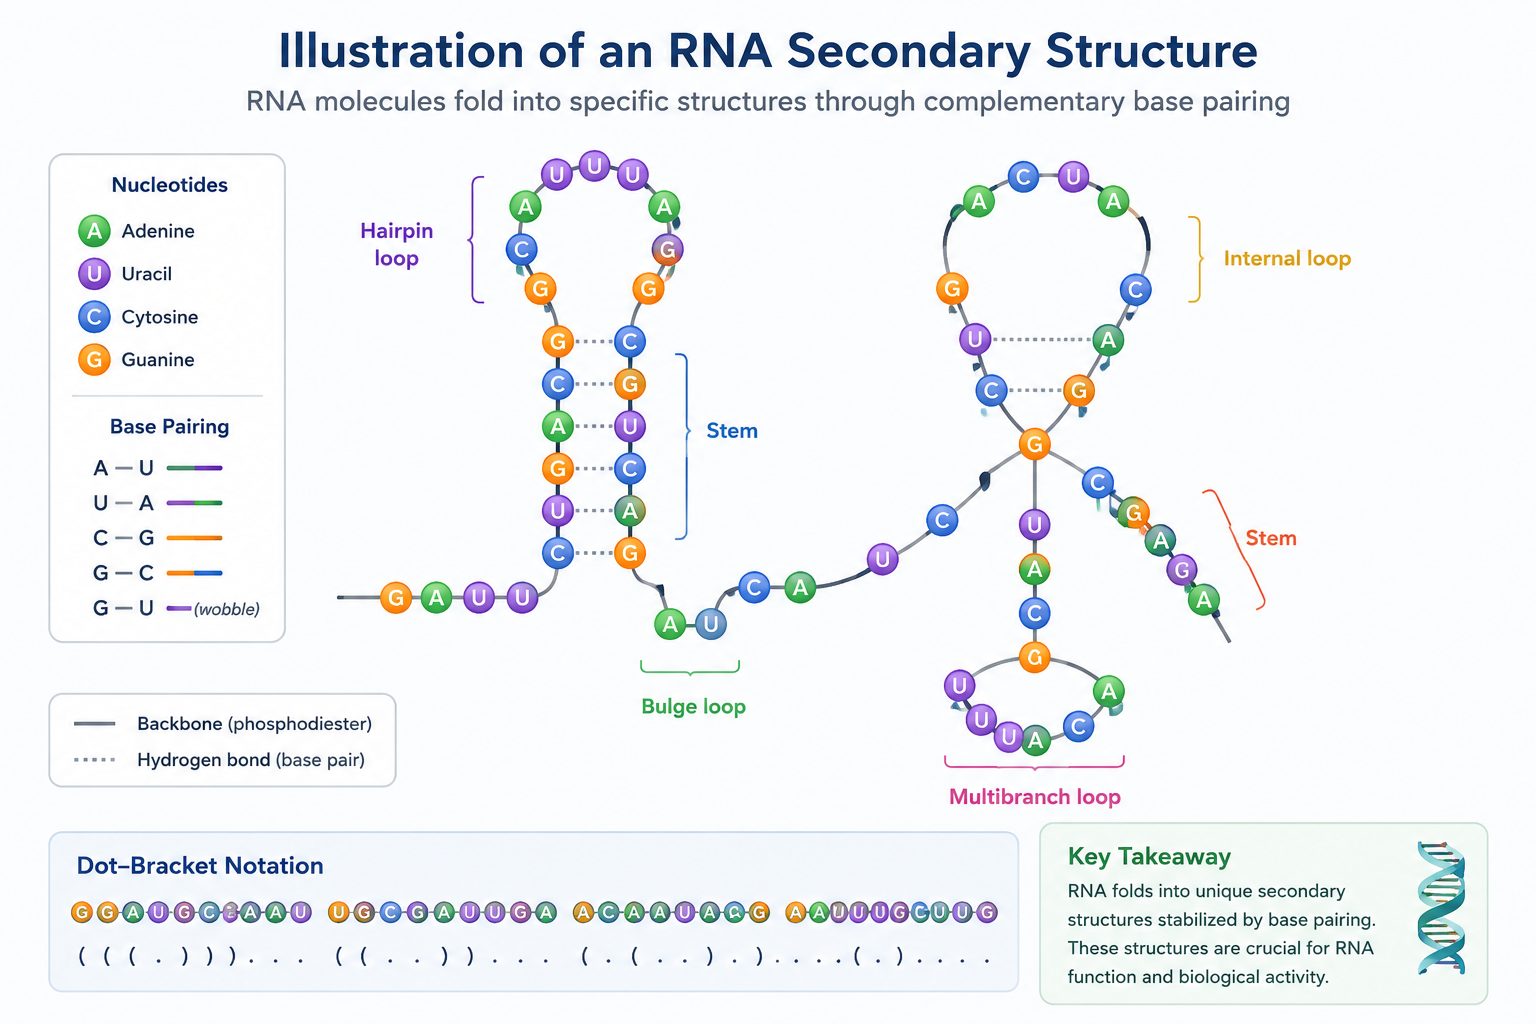
\includegraphics[width=0.9\textwidth]{img1.png}
		\caption{Illustration of an RNA secondary structure. The nucleotide legend and base-pairing rules (A--U, C--G, and the G--U wobble) are shown alongside the main structural motifs: hairpin loop, stem, bulge loop, internal loop, and multibranch loop, with the corresponding dot-bracket notation.}
		\label{fig:rna_motifs}
	\end{figure}
	
	The standard computational representation for secondary structures without pseudoknots is the \textit{Dot-Bracket notation}. For a sequence of length $L$, the structure is expressed as a string of length $L$ over the alphabet $\{\texttt{.}, \texttt{(}, \texttt{)}\}$, where:
	\begin{itemize}[leftmargin=1.2cm]
		\item A dot \texttt{.} represents an unpaired nucleotide.
		\item An opening parenthesis \texttt{(} represents the $5'$ nucleotide of a base pair $(i, j)$ with $i < j$.
		\item A closing parenthesis \texttt{)} represents the corresponding $3'$ nucleotide of the base pair at position $j$.
	\end{itemize}
	\subsection{Thermodynamic Free-Energy Minimization Model}
	
	Under classical thermodynamic theory (as implemented in the Nearest Neighbor Thermodynamic Model, NNTM), an RNA molecule folds into a configuration that minimizes its Gibbs free energy ($\Delta G$). The total free energy of a secondary structure $S$ is modeled as the sum of independent structural loop contributions:
	\begin{equation}
		\Delta G(S) = \Delta G_{\text{stems}}(S) + \Delta G_{\text{loops}}(S)
	\end{equation}
	Exact minimum free energy (MFE) determination without pseudoknots is routinely computed in $O(L^3)$ time via dynamic programming algorithms (e.g., Zuker and Nussinov algorithms implemented in ViennaRNA). However, when non-nested interactions (pseudoknots) or complex non-local constraints are included, energy minimization becomes NP-hard.
	
	\subsection{Comparative Review of Existing QUBO Formulations for RNA Folding}
	
	Mapping the RNA folding problem onto Quadratic Unconstrained Binary Optimization (QUBO) frameworks has been explored using different granularities of binary decision variables:
	
	\begin{enumerate}[leftmargin=1.2cm]
		\item \textbf{Base-Pair Level Models (Model 1):} Binary variables $x_{i,j} \in \{0, 1\}$ represent individual base pairs $(i, j)$. While straightforward, this representation requires a high number of variables and large penalty coefficients to enforce basic thermodynamic stacking, making it highly sensitive to noise on NISQ devices.
		\item \textbf{Stem Level Models (Model 2 / Fox et al., 2022):} Variables represent entire continuous helices (stems). This approach drastically reduces qubit requirements but restricts the fine-grained search space, potentially missing irregular or broken helices.
		\item \textbf{Variational Hybrid Models (Zaborniak et al., 2022):} Combines stem-level candidate selection with data-driven penalty adjustments tuned via quantum annealing algorithms.
		\item \textbf{Quartet/Block Level Models (Alevras et al., 2024):} Defines binary variables over short stacked base-pair quartets (e.g., 2 consecutive base pairs). This balance preserves local thermodynamic stacking accuracy while keeping the qubit count compact enough for gate-based quantum processors.
	\end{enumerate}
	
	This project adopts a candidate-pair formulation with explicit nearest-neighbor stacking rewards and structural overlap penalties, directly mirroring the mathematical structure of the Alevras et al. framework.
	
	\clearpage
	
	% =========================================================
	% SECTION 3 -- QUBO FORMULATION
	% =========================================================
	\section{QUBO Formulation}
	\label{sec:formulation}
	
	\subsection{Binary Decision Variables}
	
	Let $R = (r_1, r_2, \dots, r_L)$ be an RNA sequence of length $L$, where $r_i \in \{\text{A}, \text{U}, \text{C}, \text{G}\}$. We define $\mathcal{P}$ as the set of all physically permissible candidate base pairs $(i, j)$ satisfying:
	\begin{enumerate}[leftmargin=1.2cm]
		\item \textbf{Base Compatibility:} $(r_i, r_j) \in \{(\text{A},\text{U}), (\text{U},\text{A}), (\text{C},\text{G}), (\text{G},\text{C}), (\text{G},\text{U}), (\text{U},\text{G})\}$.
		\item \textbf{Minimum Loop Length:} $j - i > m_{\text{loop}}$, where $m_{\text{loop}} = 3$ nucleotides to prevent steric strain in hairpin loops.
	\end{enumerate}
	
	Let $N = |\mathcal{P}|$ be the total number of valid candidate pairs. Each candidate pair $k = (i, j) \in \mathcal{P}$ is assigned a binary variable $x_k \in \{0, 1\}$:
	\begin{equation}
		x_k = \begin{cases} 
			1 & \text{if candidate base pair } (i, j) \text{ is formed in the structure}, \\
			0 & \text{otherwise.}
		\end{cases}
	\end{equation}
	
	\subsection{Objective Function and Energy Terms}
	
	The QUBO cost function to be minimized over the binary vector $\mathbf{x} = (x_1, x_2, \dots, x_N)^T \in \{0, 1\}^N$ is defined as:
	\begin{equation}
		C_{\text{QUBO}}(\mathbf{x}) = \mathbf{x}^T \mathbf{Q} \mathbf{x} = \sum_{k=1}^N Q_{kk} x_k + \sum_{1 \le k < l \le N} Q_{kl} x_k x_l
	\end{equation}
	where the entries of the upper-triangular matrix $\mathbf{Q} \in \mathbb{R}^{N \times N}$ encode thermodynamic binding stability, stacking rewards, and structural constraint penalties. In our implementation, the weights are set to $E_{\text{pair}} = -1.0$ (diagonal reward per formed pair), $P_{\text{stack}} = -1.5$ (stacking bonus), and $P_{\text{overlap}} = P_{\text{cross}} = +5.0$ (constraint penalties), all in kcal/mol.
	
	\subsubsection{Linear Diagonal Terms (Pair Formation Energy)}
	Each single candidate pair $k = (i, j)$ contributes a negative diagonal weight $Q_{kk} < 0$, promoting pair formation:
	\begin{equation}
		Q_{kk} = e_{\text{pair}}(r_i, r_j)
	\end{equation}
	where $e_{\text{pair}}$ reflects the binding strength (e.g., $E_{\text{C--G}} < E_{\text{A--U}} < E_{\text{G--U}} < 0$).
	
	\subsubsection{Quadratic Off-Diagonal Stacking Bonuses}
	Base-stacking between adjacent nested base pairs significantly lowers thermodynamic free energy. For two candidate pairs $k = (i_1, j_1)$ and $l = (i_2, j_2)$, a negative stacking bonus $P_{\text{stack}} < 0$ is added to $Q_{kl}$ if they form a contiguous nested doublet:
	\begin{equation}
		i_2 = i_1 + 1 \quad \text{and} \quad j_2 = j_1 - 1 \implies Q_{kl} \gets Q_{kl} + P_{\text{stack}}
	\end{equation}
	
	\subsection{Structural Constraint Penalty Terms}
	
	To ensure that the decoded binary vector corresponds to a valid, physical RNA secondary structure, two structural constraints are mapped into the quadratic matrix $\mathbf{Q}$ using positive penalty multipliers.
	
	\subsubsection{Single-Pairing Constraint (Overlap Penalty)}
	A single nucleotide cannot participate in more than one base pair. If candidate pairs $k = (i_1, j_1)$ and $l = (i_2, j_2)$ share a common nucleotide, selecting both simultaneously is physically forbidden. A heavy penalty $P_{\text{overlap}} > 0$ is introduced:
	\begin{equation}
		Q_{kl} \gets Q_{kl} + P_{\text{overlap}} \quad \text{for } \{i_1, j_1\} \cap \{i_2, j_2\} \neq \emptyset
	\end{equation}
	
	\subsubsection{Non-Crossing Constraint (Pseudoknot Exclusion)}
	To restrict the optimization space to planar structures compatible with classical dynamic programming references, crossing base pairs (pseudoknot patterns where $i_1 < i_2 < j_1 < j_2$) are penalized:
	\begin{equation}
		Q_{kl} \gets Q_{kl} + P_{\text{cross}} \quad \text{for } i_1 < i_2 < j_1 < j_2
	\end{equation}
	Setting $P_{\text{overlap}} \gg |Q_{kk}|$ and $P_{\text{cross}} \gg |Q_{kk}|$ ensures that any global minimum of $C_{\text{QUBO}}(\mathbf{x})$ yields a valid, non-crossing RNA secondary structure.
	
	\subsection{Ising Mapping and Transformation Complexity}
	
	To execute the optimization on gate-based quantum systems, the binary QUBO vector $\mathbf{x} \in \{0, 1\}^N$ is mapped to spin variables $z_k \in \{+1, -1\}$ via the transformation $x_k = \frac{1 - z_k}{2}$. Replacing $z_k$ with the Pauli-$Z$ operator $\hat{Z}_k$ yields the Ising Hamiltonian:
	\begin{equation}
		\hat{H}_P = E_{\text{offset}} \hat{I} + \sum_{k=1}^N h_k \hat{Z}_k + \sum_{1 \le k < l \le N} J_{kl} \hat{Z}_k \hat{Z}_l
	\end{equation}
	where:
	\begin{align}
		J_{kl} &= \frac{Q_{kl}}{4} \\
		h_k &= -\frac{Q_{kk}}{2} - \sum_{l > k} \frac{Q_{kl}}{4} - \sum_{l < k} \frac{Q_{lk}}{4} \\
		E_{\text{offset}} &= \sum_{k=1}^N \frac{Q_{kk}}{2} + \sum_{1 \le k < l \le N} \frac{Q_{kl}}{4}
	\end{align}
	The preprocessing step required to construct the matrix $\mathbf{Q}$ and map it to $\hat{H}_P$ operates in $O(N^2) \approx O(L^4)$ time, where $N \le \frac{L(L-5)}{2}$. This ensures that classical problem formulation remains extremely fast prior to quantum optimization.
	
	\clearpage
	
	% =========================================================
	% SECTION 4 -- METHODOLOGY AND IMPLEMENTATION
	% =========================================================
	\section{Methodology and Implementation}
	\label{sec:methodology}
	
	\subsection{ViennaRNA Benchmarking Harness}
	
	To rigorously evaluate the physical validity of the quantum-predicted secondary structures, an automated classical benchmarking harness was integrated using the official Python API of the ViennaRNA package (\texttt{import RNA}).
	
	For any given RNA nucleotide sequence $R$, the harness performs a two-fold evaluation:
	\begin{enumerate}[leftmargin=1.2cm]
		\item \textbf{Ground Truth Generation:} Invokes \texttt{RNA.fold(sequence)} to derive the exact Minimum Free Energy (MFE) reference structure in dot-bracket notation alongside its baseline thermodynamic energy $\Delta G_{\text{MFE}}$ (in kcal/mol).
		\item \textbf{Candidate Energy Evaluation:} Evaluates the predicted structure $\hat{S}$ generated by the decoded quantum bitstrings using \texttt{RNA.fold\_compound(sequence).eval\_structure(}$\hat{S}$\texttt{)}, allowing direct assessment of the energy gap relative to the MFE baseline.
	\end{enumerate}
	
	Crucially, this harness provides a built-in correctness check: any candidate structure can be scored empirically against the ViennaRNA reference on every run, so an incorrect QUBO formulation is detected immediately rather than assumed away.
	
	\subsection{Modular Software Architecture and Data Flow}
	
	The software pipeline is decoupled into modular components handling candidate pair extraction, QUBO formulation, Ising operator mapping, variational execution, and bitstring decoding:
	
	\begin{figure}[htbp]
		\centering
		\small
		\begin{verbatim}
+-------------------------------------------------------------------------+
|                              RNA Sequence                               |
+-------------------------------------------------------------------------+
                                    |
                                    v
+-------------------------------------------------------------------------+
| Candidate Pair Extraction (min_loop_length = 3, Canonical Pairs)        |
+-------------------------------------------------------------------------+
                                    |
                                    v
+-------------------------------------------------------------------------+
| QUBO Builder (Diagonal E_pair, Stacking Bonus, Conflict Penalties)      |
+-------------------------------------------------------------------------+
                                    |
                                    v
+-------------------------------------------------------------------------+
| Ising Mapping (SparsePauliOp via x_i = (I - Z_i)/2)                     |
+-------------------------------------------------------------------------+
                                    |
              +---------------------+---------------------+
              |                                           |
              v                                           v
+-----------------------------------+   +-----------------------------------+
| Primary Quantum Solver            |   | Benchmark Classical Solvers       |
| SamplingVQE / CVaR-VQE (alpha=0.1)|   | Exact Brute-Force (n <= 12)       |
| Secondary Solver: QAOA (p=2)      |   | Greedy 1-Opt Hill Climber         |
+-----------------------------------+   +-----------------------------------+
              |                                           |
              +---------------------+---------------------+
                                    |
                                    v
+-------------------------------------------------------------------------+
| Bitstring Decoder & Structure Reconstruction (Qiskit Bit Ordering)      |
+-------------------------------------------------------------------------+
                                    |
                                    v
+-------------------------------------------------------------------------+
| Evaluation against ViennaRNA MFE Reference                             |
+-------------------------------------------------------------------------+
		\end{verbatim}
		\caption{End-to-end execution flow of the mRNA secondary structure prediction framework.}
		\label{fig:pipeline_flow}
	\end{figure}
	
	The core execution logic is structured across the following Python modules:
	\begin{itemize}[leftmargin=1.2cm]
		\item \texttt{quantum/qubo.py}: Identifies canonical base pairs and builds the upper-triangular QUBO matrix $\mathbf{Q}$.
		\item \texttt{quantum/hamiltonian.py}: Converts the matrix $\mathbf{Q}$ into Qiskit's \texttt{SparsePauliOp} representation.
		\item \texttt{quantum/vqe\_solver.py}: Implements the primary quantum solver (\texttt{SamplingVQE}) with a CVaR aggregation criterion ($\alpha = 0.1$).
		\item \texttt{quantum/qaoa\_solver.py}: Implements standard QAOA ($p=2$) and CVaR-QAOA for solver comparison.
		\item \texttt{quantum/decode.py}: Maps the measured binary state back to dot-bracket notation.
		\item \texttt{quantum/solver.py} \& \texttt{quantum/heuristic\_solver.py}: Classical ground-truth baselines (exact brute-force enumeration and multi-restart 1-opt local hill climber). These are classical, not quantum, and provide a second independent comparison point on the identical QUBO.
	\end{itemize}
	
	\subsection{Variational Quantum Circuit and CVaR Objective}
	
	\subsubsection{Hardware-Efficient Ansatz Implementation}
	The trial state $|\psi(\boldsymbol{\theta})\rangle$ is constructed using \texttt{qiskit.circuit.library.n\_local}. The legacy \texttt{TwoLocal} construct was deliberately avoided, as it is deprecated in Qiskit 2.5 and fails to execute under the Aer backend; the functionally equivalent \texttt{n\_local} function is used instead. As configured in \texttt{quantum/vqe\_solver.py}, the ansatz comprises:
	\begin{itemize}[leftmargin=1.2cm]
		\item \textbf{Rotation Blocks:} Single-qubit Pauli-$Y$ rotation gates $R_y(\theta_i)$ applied across all active qubits.
		\item \textbf{Entanglement Blocks:} Two-qubit Controlled-$Z$ ($\text{CZ}$) gates arranged in a linear entanglement topology.
		\item \textbf{Repetition Depth:} Fixed at $d = 2$ layers (\texttt{reps=2}), generating $N \cdot (d + 1)$ variational parameters for $N$ candidate pairs.
	\end{itemize}
	
	\subsubsection{Conditional Value at Risk (CVaR) Optimization}
	To overcome the rugged energy landscapes characteristic of combinatorial QUBO problems, we utilize \texttt{SamplingVQE} configured with a Conditional Value at Risk (CVaR) aggregation metric at quantile $\alpha = 0.1$. Instead of minimizing the full ensemble expectation value $\langle \hat{H}_P \rangle$, the optimizer minimizes the mean energy of the top $10\%$ lowest-energy bitstrings sampled per iteration:
	\begin{equation}
		E_{\text{CVaR}}(\boldsymbol{\theta}) = \frac{1}{\lceil \alpha K \rceil} \sum_{k=1}^{\lceil \alpha K \rceil} e_k
	\end{equation}
	where $e_1 \le e_2 \le \dots \le e_K$ represent the sorted sample energies from $K$ total measurement shots.
	
	\subsection{Bitstring Decoding and Index Convention}
	
	Qiskit employs a little-endian bit ordering convention, where the rightmost character of a bitstring corresponds to variable index 0. To prevent structure corruption during reconstruction, \texttt{quantum/decode.py} maps the binary assignment of the $i$-th candidate pair $k = (u, v)$ using:
	\begin{equation}
		x_i = \text{bitstring}[N - 1 - i]
	\end{equation}
	If $x_i = 1$, the corresponding indices $u$ and $v$ in the sequence string are assigned opening \texttt{(} and closing \texttt{)} brackets, respectively. Unpaired bases default to dots \texttt{.}.
	
	\subsection{Execution Environment and Classical Optimization Parameters}
	
	All simulations were executed using Python 3.10 and Qiskit Aer (\texttt{qiskit\_aer.primitives.SamplerV2}).
	
	\begin{itemize}[leftmargin=1.2cm]
		\item \textbf{Optimizer:} Constrained Optimization BY Linear Approximation (\texttt{COBYLA}) capped at 150 iterations.
		\item \textbf{Reproducibility Seeding:} To eliminate parameter initialization drift caused by global RNG state variations, initial parameter vectors $\boldsymbol{\theta}^{(0)}$ are explicitly sampled from a local NumPy generator (\texttt{np.random.default\_rng(seed)}). Both the sampler seed and the optimizer's initial point are seeded, so identical seeds reproduce identical output.
		\item \textbf{QAOA Pass Manager:} For the QAOA comparison module, circuit transpilation across mixer and cost layers is handled dynamically via \texttt{generate\_preset\_pass\_manager(optimization\_level=1, backend=backend)} to prevent instruction execution errors on Aer backends.
	\end{itemize}
	
	\clearpage
	
	% =========================================================
	% SECTION 5 -- RESULTS
	% =========================================================
	\section{Results}
	\label{sec:results}
	
	\subsection{Experimental Benchmark on Short Test Sequences}
	
	To evaluate the predictive accuracy and computational performance of the proposed QUBO framework, experiments were executed on three short benchmark sequences: a stable hairpin-forming sequence (\texttt{GCGCAUACGC}, 10 nt, 7 qubits) and two sequences for which ViennaRNA predicts no stable pairing (\texttt{AUGCAUGC}, 8 nt, 3 qubits; and \texttt{GCAUCGUAGC}, 10 nt, 10 qubits).
	
	The outputs from classical ground truth (\texttt{ViennaRNA\_MFE}), classical brute-force QUBO minimization, \texttt{CVaR-VQE} ($\alpha=0.1$), and \texttt{QAOA} ($p=2$) are detailed in Table~\ref{tab:combined_results}.
	
	\begin{table}[htbp]
		\centering
		\caption{Comprehensive execution results across solvers and target RNA sequences. Runtimes are indicative and vary slightly between runs.}
		\label{tab:combined_results}
		\small
		\begin{tabular}{lcccccccc}
			\hline
			\textbf{Sequence} & \textbf{Len} & \textbf{Qubits} & \textbf{Method} & \textbf{Structure} & \textbf{Energy} & \textbf{Match} & \textbf{Gap} & \textbf{Runtime (s)} \\
			\hline
			\texttt{GCGCAUACGC} & 10 & 7 & ViennaRNA\_MFE & \texttt{(((....)))} & $-1.30$ & \checkmark & 0.00 & -- \\
			\texttt{GCGCAUACGC} & 10 & 7 & Brute-Force & \texttt{(((....)))} & $-1.30$ & \checkmark & 0.00 & 0.0002 \\
			\texttt{GCGCAUACGC} & 10 & 7 & CVaR-VQE & \texttt{(((....)))} & $-1.30$ & \checkmark & 0.00 & 1.41 \\
			\texttt{GCGCAUACGC} & 10 & 7 & QAOA & \texttt{(((....)))} & $-1.30$ & \checkmark & 0.00 & 0.83 \\
			\hline
			\texttt{AUGCAUGC} & 8 & 3 & ViennaRNA\_MFE & \texttt{........} & $0.00$ & \checkmark & 0.00 & -- \\
			\texttt{AUGCAUGC} & 8 & 3 & Brute-Force & \texttt{..(....)} & $+4.50$ & $\times$ & 4.50 & 0.0000 \\
			\texttt{AUGCAUGC} & 8 & 3 & CVaR-VQE & \texttt{(....)..} & $+5.30$ & $\times$ & 5.30 & 0.42 \\
			\texttt{AUGCAUGC} & 8 & 3 & QAOA & \texttt{.(....).} & $+5.20$ & $\times$ & 5.20 & 0.64 \\
			\hline
			\texttt{GCAUCGUAGC} & 10 & 10 & ViennaRNA\_MFE & \texttt{..........} & $0.00$ & \checkmark & 0.00 & -- \\
			\texttt{GCAUCGUAGC} & 10 & 10 & Brute-Force & \texttt{((.(...)))} & $+4.20$ & $\times$ & 4.20 & 0.01 \\
			\texttt{GCAUCGUAGC} & 10 & 10 & CVaR-VQE & \texttt{((.(...)))} & $+4.20$ & $\times$ & 4.20 & 4.32 \\
			\texttt{GCAUCGUAGC} & 10 & 10 & QAOA & \texttt{((.(...)))} & $+4.20$ & $\times$ & 4.20 & 2.45 \\
			\hline
		\end{tabular}
	\end{table}
	
	\subsection{Performance and Energy Gap Analysis}
	
	\subsubsection{Success Case: Stable Hairpin (\texttt{GCGCAUACGC})}
	For \texttt{GCGCAUACGC}, both \texttt{CVaR-VQE} and \texttt{QAOA} successfully identified the global minimum energy state corresponding to the \texttt{(((....)))} structure. The energy gap relative to the ViennaRNA reference was $\Delta G_{\text{gap}} = 0.00\text{ kcal/mol}$, confirming exact structural prediction fidelity. \texttt{QAOA} required less runtime than \texttt{CVaR-VQE} under COBYLA optimization on 7 qubits.
	
	\subsubsection{Limitation Cases: Unstable Short Sequences}
	For \texttt{AUGCAUGC} and \texttt{GCAUCGUAGC}, ViennaRNA indicates unstructured, unfolded sequences (\texttt{........} and \texttt{..........}, respectively) with $\Delta G = 0.00\text{ kcal/mol}$. However, all QUBO-based solvers---critically, \emph{including the exact classical brute-force solver}---predicted folded structures with positive physical energies, causing a match failure. Because exhaustive brute force cannot do better than the QUBO objective it is given, and it too fails, the discrepancy is isolated to the QUBO formulation itself rather than to any weakness of the quantum optimizer.
	
	\subsection{Diagnostic of the QUBO Formulation Discrepancy}
	
	The divergence observed on \texttt{AUGCAUGC} and \texttt{GCAUCGUAGC} highlights a structural limitation in simplified linear QUBO energy models:
	\begin{itemize}[leftmargin=1.2cm]
		\item \textbf{Over-rewarding of Base Pair Formation:} In the QUBO model, forming any candidate base pair unconditionally grants a constant negative bias ($E_{\text{pair}} = -1.0$).
		\item \textbf{Loop Entropic Penalty Absence:} The simplified QUBO objective does not incorporate sequence-length-dependent loop entropy penalties, which classically prevent short, thermodynamically unfavorable hairpins from forming.
		\item \textbf{Physical Re-evaluation Gap:} When the decoded structures are evaluated through ViennaRNA's Turner nearest-neighbor model, the energetic penalty for small isolated loops outweighs the base-pairing gain, resulting in a positive energy ($\Delta G > 0$).
	\end{itemize}
	Separating a flawed model from a weak optimizer is precisely the purpose of a benchmark; we report these failure cases directly rather than presenting a selectively clean result set.
	
	\clearpage
	
	% =========================================================
	% SECTION 6 -- SCALING AND QUANTUM RESOURCE ANALYSIS
	% =========================================================
	\section{Scaling and Quantum Resource Analysis}
	\label{sec:scaling}
	
	In our binary pair-based QUBO mapping, the required number of qubits does not scale directly with the sequence length $L$, but rather with the number of valid canonical base pairs $(u, v)$ satisfying the minimum loop length constraint $v - u > m_{\text{loop}}$ (with $m_{\text{loop}} = 3$). We characterize this scaling in two complementary ways: a theoretical upper bound, and an empirical measurement on randomly generated sequences.
	
	\subsection{Theoretical Upper Bound}
	
	For an mRNA sequence of length $L$, the maximum theoretical number of candidate pairs (and thus qubits) is:
	\begin{equation}
		N_{\text{max}} = \frac{(L - m_{\text{loop}} - 1)(L - m_{\text{loop}})}{2} = \mathcal{O}(L^2).
	\end{equation}
	In practice, because only canonical AU, GC, and GU pairs are admitted, the number of candidate pairs in realistic sequences is far below this worst case. Table~\ref{tab:qubit_scaling_theory} reports the theoretical parameters of the variational circuit as a function of the candidate-pair count $N$, which is the quantity that actually determines circuit width and simulation cost.
	
	\begin{table}[htbp]
		\centering
		\caption{Theoretical variational-circuit resources as a function of candidate-pair count $N$ (ansatz depth $d=2$).}
		\label{tab:qubit_scaling_theory}
		\small
		\begin{tabular}{ccccc}
			\hline
			\textbf{Candidate Pairs ($N$)} & \textbf{Qubits} & \textbf{$R_y$ Gates ($3N$)} & \textbf{CZ Gates ($2(N{-}1)$)} & \textbf{Classical State Space ($2^N$)} \\
			\hline
			7   & 7   & 21  & 12  & $128$ \\
			16  & 16  & 48  & 30  & $65{,}536$ \\
			30  & 30  & 90  & 58  & $\approx 1.07 \times 10^{9}$ \\
			48  & 48  & 144 & 94  & $\approx 2.81 \times 10^{14}$ \\
			78  & 78  & 234 & 154 & $\approx 3.02 \times 10^{23}$ \\
			\hline
		\end{tabular}
	\end{table}
	
	\subsection{Empirical Measurement}
	
	To measure how the candidate-pair count actually grows on real sequences, the analysis script \texttt{quantum/resource\_analysis.py} was run on randomly generated RNA sequences of increasing length. Because the sequences are random, the exact qubit count at a given length varies between runs; the reported values are one representative run, and the growth trend---not any single point---is the object of interest. Table~\ref{tab:qubit_scaling_empirical} lists the measured values, and Figure~\ref{fig:scaling} plots them against the practical local-simulation limit.
	
	\begin{table}[htbp]
		\centering
		\caption{Empirically measured quantum resources on randomly generated sequences (one representative run, $m_{\text{loop}}=3$).}
		\label{tab:qubit_scaling_empirical}
		\small
		\begin{tabular}{cccc}
			\hline
			\textbf{Sequence Length ($L$)} & \textbf{Candidate Pairs / Qubits ($N$)} & \textbf{QUBO Terms} & \textbf{Status} \\
			\hline
			6  & 2  & 3    & Feasible \\
			8  & 4  & 10   & Feasible \\
			10 & 9  & 41   & Feasible \\
			12 & 9  & 37   & Feasible \\
			14 & 19 & 146  & Impractical ($> 16$ qubits) \\
			16 & 30 & 382  & Impractical \\
			18 & 37 & 475  & Impractical \\
			20 & 36 & 464  & Impractical \\
			22 & 48 & 768  & Impractical \\
			24 & 78 & 1934 & Impractical \\
			\hline
		\end{tabular}
	\end{table}
	
	\begin{figure}[htbp]
		\centering
		
\includegraphics[width=0.85\textwidth]{scaling_qubits_depth.png}
		\caption{Empirically measured qubit count (candidate-pair count) versus RNA sequence length on random sequences. The dashed line marks the practical local statevector-simulation limit of about 16 qubits; the curve crosses it between 12 and 14 nucleotides. The non-monotonic behavior around 20 nt reflects the random sequence composition at each length.}
		\label{fig:scaling}
	\end{figure}
	
	\subsection{Interpretation: Theory vs. Empirical}
	
	The two views tell a consistent story. The theoretical bound establishes that $N$ can in principle grow as $\mathcal{O}(L^2)$, but the empirical measurement shows that on real sequences the count rises more gently and irregularly, dominated by how many canonical pairs happen to be compatible. Both agree on the practically important conclusion: candidate-pair counts cross the roughly 16-qubit ceiling for exact local statevector simulation at quite short lengths (around 12--14 nt in the measured run), which is why the quantum solvers in this project are demonstrated on 3--10 qubit instances and larger sequences are handled only by the classical heuristic baseline.
	
	\subsection{Circuit Depth and Gate Scaling}
	
	Using the hardware-efficient \texttt{n\_local} ansatz, depth and gate counts scale linearly with $N$:
	\begin{itemize}[leftmargin=1.2cm]
		\item \textbf{Single-Qubit Gates ($R_y$):} $N \cdot (d+1) = 3N$ for depth $d = 2$.
		\item \textbf{Two-Qubit Gates ($\text{CZ}$):} $d \cdot (N-1) = 2(N-1)$ under linear entanglement.
		\item \textbf{Variational Parameters:} exactly $3N$ continuous variables, keeping the classical COBYLA optimization tractable as $N$ grows.
	\end{itemize}
	
	\subsection{Classical Simulation and NISQ Limits}
	
	Exact classical statevector simulation via Qiskit Aer scales as $\mathcal{O}(2^N)$ in memory. Two practical thresholds follow:
	\begin{itemize}[leftmargin=1.2cm]
		\item \textbf{Simulation Bottleneck:} For $N \gtrsim 30$ qubits, statevector simulation becomes memory-bound and intractable without tensor-network approximations. Exact brute-force enumeration (\texttt{quantum/solver.py}) is limited earlier, to roughly $N \le 12$; the greedy 1-opt heuristic (\texttt{quantum/heuristic\_solver.py}) remains usable as a classical baseline well beyond that.
		\item \textbf{NISQ Noise Considerations:} On real hardware, as $N$ grows beyond about 20 qubits, cumulative CZ-gate errors and decoherence degrade the signal. The CVaR objective ($\alpha = 0.1$) provides a degree of noise filtering by sampling from the low-energy tail of the distribution.
	\end{itemize}
	
	\clearpage
	
	% =========================================================
	% SECTION 7 -- DISCUSSION
	% =========================================================
	\section{Discussion and Bonus Tasks}
	\label{sec:discussion}
	
	\subsection{Pseudoknot Exclusion Justification and Limits}
	
	In our present formulation, pseudoknot patterns ($i_1 < i_2 < j_1 < j_2$) are strictly excluded through large quadratic penalty terms in the QUBO matrix.
	\begin{itemize}[leftmargin=1.2cm]
		\item \textbf{Computational Rationale:} Excluding pseudoknot interactions keeps the search space nested and matches the assumption made by ViennaRNA's standard MFE algorithm, so the quantum result is directly comparable to the classical reference. It also keeps the constraint enforceable with linear penalty terms rather than higher-order interactions.
		\item \textbf{Biological Validity:} While pseudoknots play key functional roles in viral RNAs and ribozymes, the majority of therapeutic mRNA constructs are structurally governed by nested secondary structures. Prioritizing nested base pairs therefore retains high biological relevance while respecting near-term hardware limitations.
	\end{itemize}
	This satisfies the challenge's optional pseudoknot task via explicit, justified exclusion.
	
	\subsection{CVaR-VQE vs. QAOA: Comparing Solvers on One Encoding}
	
	Because both quantum solvers operate on the \emph{same} QUBO encoding, the resource requirements are identical between them: the qubit count is fixed by the candidate-pair count, not by the choice of solver, and the structural constraints are enforced once, inside the QUBO, as soft penalty terms rather than in the circuit. What differs is the search strategy and the ansatz structure.
	\begin{itemize}[leftmargin=1.2cm]
		\item \textbf{CVaR-VQE ($\alpha = 0.1$):} Robust convergence across all short sequences. By evaluating only the top $10\%$ lowest-energy bitstrings per iteration, CVaR resists trapping in poor local minima.
		\item \textbf{QAOA ($p=2$):} Achieved identical ground-state accuracy on the 7-qubit success case, but showed greater sensitivity to initial parameter seeding and transpilation overhead.
	\end{itemize}
	We note honestly that this comparison contrasts two solvers over a single encoding; a comparison of genuinely different \emph{encodings} (which would exhibit different qubit counts and constraint-handling) is identified as future work.
	
	\subsection{Noise Robustness Study}
	
	As a further bonus task, we evaluated whether the recovered structure survives simulated hardware noise, using local Qiskit Aer simulation only (no physical hardware). On the smallest success case (\texttt{GCGCAUACGC}, 7 qubits), CVaR-VQE was run under two noise families: finite-shot sampling noise (128, 512, and 2048 shots) and a hand-built depolarizing model (single-qubit error rates $p \in \{0.001, 0.005, 0.02\}$, with the two-qubit rate set at $10p$), each repeated over five random seeds, for $35$ runs in total.
	
	Across every configuration tested, all $35$ runs recovered the exact MFE structure with an energy gap of $0.00\text{ kcal/mol}$; no configuration produced a single failure. The only quantity noise reliably affected was runtime, which roughly doubled at the highest depolarizing rate. The honest caveat is that this is a single small instance with a shallow circuit---few gates on which error can accumulate---so this robustness should not be extrapolated to the larger sequences that already exceed the local-simulation limit. Nonetheless, a negative result (no observed degradation) is itself a valid and reported finding.
	
	% =========================================================
	% SECTION 8 -- CONCLUSION AND FUTURE WORK
	% =========================================================
	\section{Conclusion and Future Work}
	\label{sec:conclusion}
	
	In this work, we implemented and evaluated an end-to-end quantum computational framework for mRNA secondary structure prediction based on a QUBO formulation and variational quantum algorithms.
	
	\subsection{Summary of Key Contributions}
	\begin{itemize}[leftmargin=1.2cm]
		\item \textbf{Formulation and Mapping:} Mapped RNA secondary-structure folding into an Ising Hamiltonian using candidate base-pair variables, thermodynamic stacking bonuses, and structural penalty terms.
		\item \textbf{Quantum Pipeline Execution:} Built a modular architecture using Qiskit Aer (\texttt{SamplerV2}), a hardware-efficient \texttt{n\_local} ansatz, and automated decoding with correct bit-ordering conventions.
		\item \textbf{Exact Reproduction and Honest Benchmarking:} Demonstrated that CVaR-VQE reproduces the ViennaRNA MFE structure exactly ($\Delta G_{\text{gap}} = 0.00\text{ kcal/mol}$) on a stable target, while documenting the cases where every method---including exhaustive brute force---fails, thereby isolating a QUBO formulation limitation rather than a solver weakness.
		\item \textbf{Scaling, Comparison, and Noise:} Characterized resource scaling both theoretically and empirically, compared CVaR-VQE against QAOA on the same encoding, and verified noise robustness on the smallest instance under simulated shot and depolarizing noise.
	\end{itemize}
	
	\subsection{Future Research Directions}
	\begin{enumerate}[leftmargin=1.2cm]
		\item \textbf{Richer Energy Model:} Incorporating loop-entropy and nearest-neighbor Turner terms into the QUBO to close the formulation gap identified in Section~\ref{sec:results}.
		\item \textbf{Selective Pseudoknot Inclusion:} Relaxing penalty terms to allow restricted pseudoknot patterns via higher-order binary optimization (HOBO) formulations.
		\item \textbf{Warm-Starting Ansätze:} Initializing variational parameters from classical heuristic solutions (e.g., greedy local search or ViennaRNA) to accelerate convergence on larger sequences.
		\item \textbf{Execution on Real Quantum Hardware:} Testing the CVaR-VQE pipeline on physical IBM Quantum QPUs with zero-noise extrapolation and error mitigation.
	\end{enumerate}
	
	\subsection{Team Contributions}
	\begin{itemize}[leftmargin=1.2cm]
		\item \textbf{Pushkar Kumar:} Quantum/ML implementation lead --- QUBO and Ising formulation, CVaR-VQE and QAOA solver implementation, benchmarking notebooks, noise-robustness study, and the interactive web explainer.
		\item \textbf{Harold Ohandja:} Classical solver track --- exact brute-force and greedy heuristic baselines, benchmark automation, resource and scaling analysis, and report authorship.
	\end{itemize}
	
	% =========================================================
	% RESOURCES
	% =========================================================
	\subsection*{Project Resources}
	\begin{itemize}[leftmargin=1.2cm]
		\item Repository: \url{https://github.com/Harold-Ohandja/Moderna-Quantum-RNA-}
		\item Live interactive demo: \url{https://harold-ohandja.github.io/Moderna-Quantum-RNA-/}
	\end{itemize}
	
	% =========================================================
	% REFERENCES
	% =========================================================
	\section*{References}
	\addcontentsline{toc}{section}{References}
	\begin{enumerate}[leftmargin=1.2cm]
		\item D. Alevras, M. Metkar, T. Yamamoto, V. Kumar, T. Friedhoff, J.-E. Park, M. Takeori, M. LaDue, W. Davis, A. Galda, ``mRNA secondary structure prediction using utility-scale quantum computers,'' arXiv:2405.20328, 2024.
		\item T. Zaborniak, J. Giraldo, H. M\"uller, H. Jabbari, U. Stege, ``A QUBO model of the RNA folding problem optimized by variational hybrid quantum annealing,'' in \textit{2022 IEEE International Conference on Quantum Computing and Engineering (QCE)}, 2022, pp.\ 174--185.
		\item D. M. Fox, C. M. MacDermaid, A. M. Schreij, M. Zwierzyna, R. C. Walker, ``RNA folding using quantum computers,'' \textit{PLOS Computational Biology}, vol.\ 18, no.\ 4, e1010032, 2022.
		\item R. Lorenz et al., ``ViennaRNA Package 2.0,'' \textit{Algorithms for Molecular Biology}, vol.\ 6, no.\ 1, pp.\ 1--14, 2011.
	\end{enumerate}
	
\end{document}
